\newpage
\section{Process}

\subsection{Sekvensdiagrammer}
Der er udarbejdet et sekvensdiagram for hver use case. Sekvensdiagramerne beskriver hvordan systemets dele og aktører interagerer med hinanden, og hvilke processer der sker ved disse interaktioner. 
For at simplificere store sekvensdiagrammer gør nogle af dem brug af andre use cases, dette ses fx. i sekvensdiagrammet for use case 1. 


\newpage
\subsection{Konditionering - UC1} 
\hspace{2cm}
{\pdfpagewidth=2\pdfpagewidth
	\vspace*{-2cm}
	\noindent\kern.5\pdfpagewidth\rlap{\parbox{\textwidth}{%
			\noindent\kern.25\pdfpagewidth
			\llap{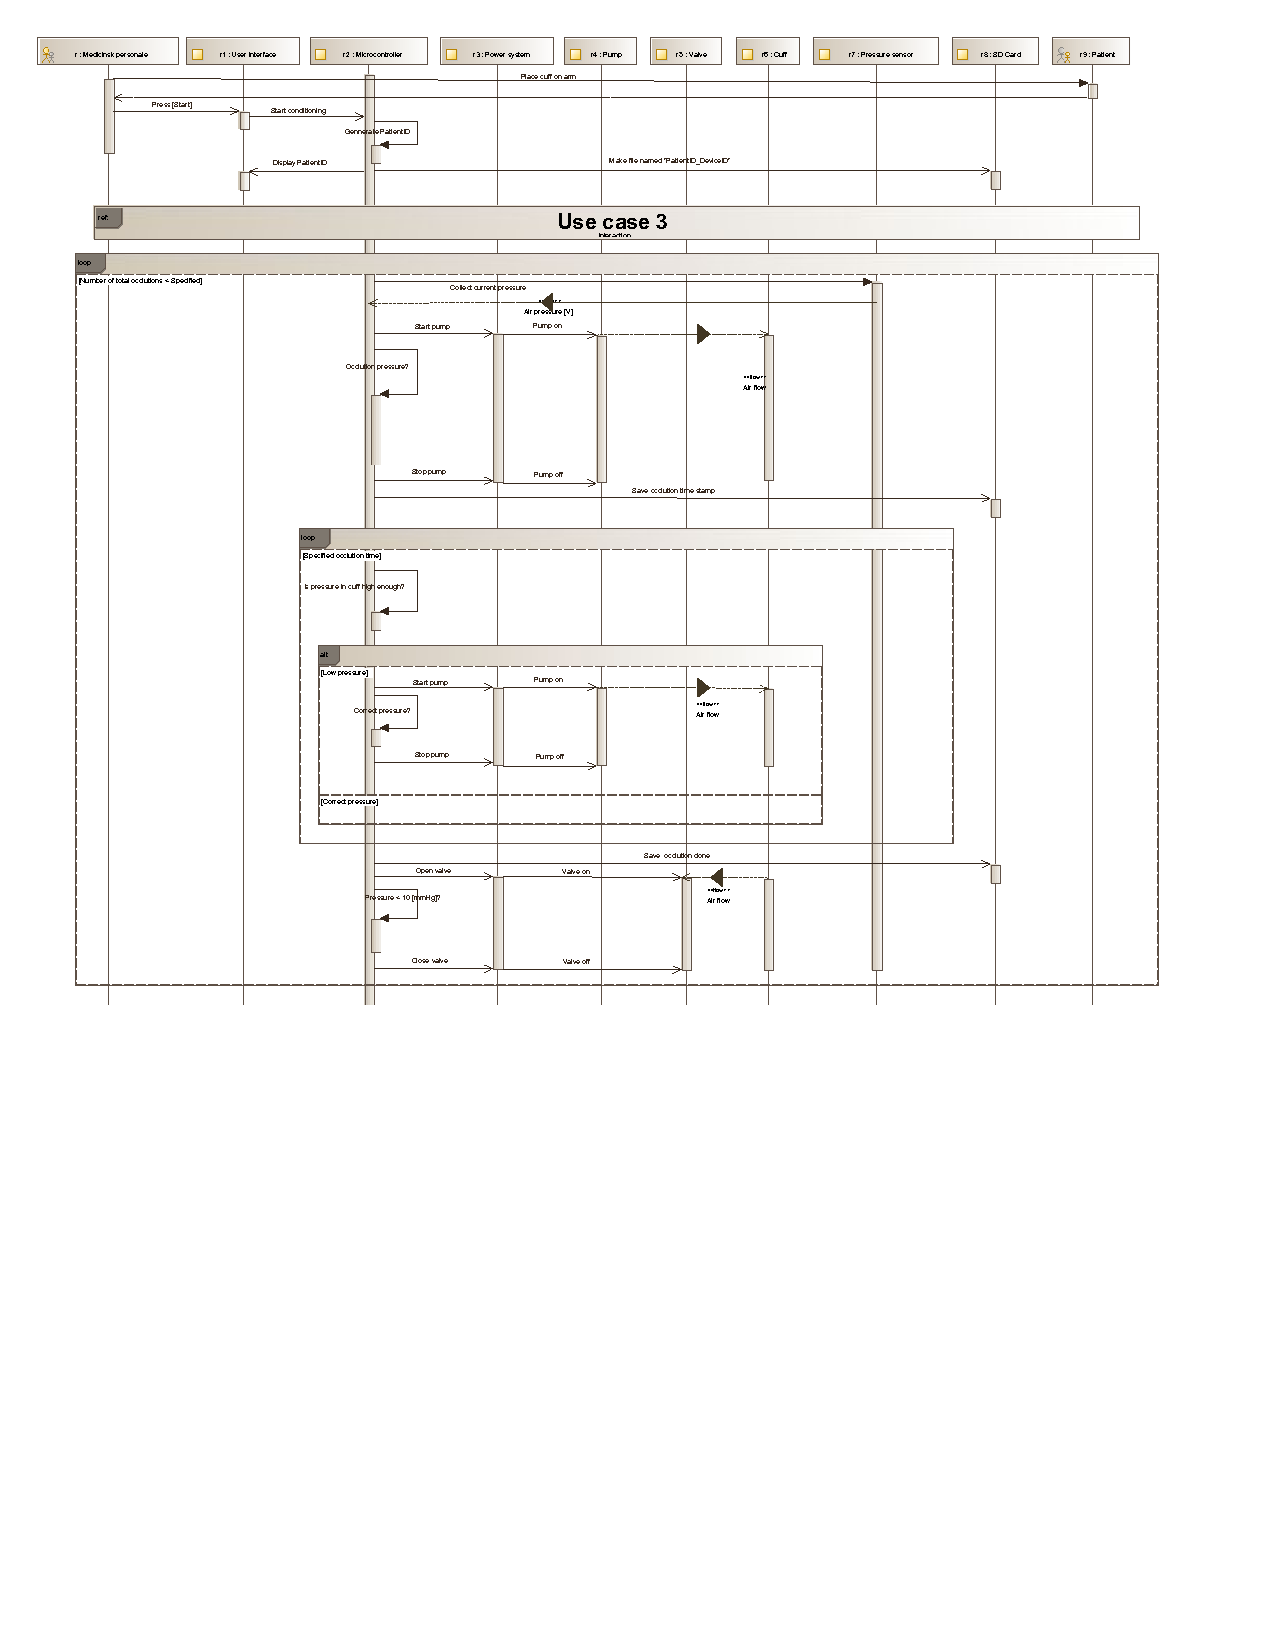
\includegraphics[width=308mm,height=229mm,page=1]{SystemArkitektur/pdfs/SD_UC1-crop.pdf}}\endgraf
			\vspace{2ex}%
			\captionof{figure}{Sekvens diagram over forløb i use case 1}}}\kern-.5\pdfpagewidth
	\par
	\vspace*{-5cm}
	\clearpage
}
\newpage

\subsection{Initialiser blodtryksmåling - UC2}
\begin{figure}[H]
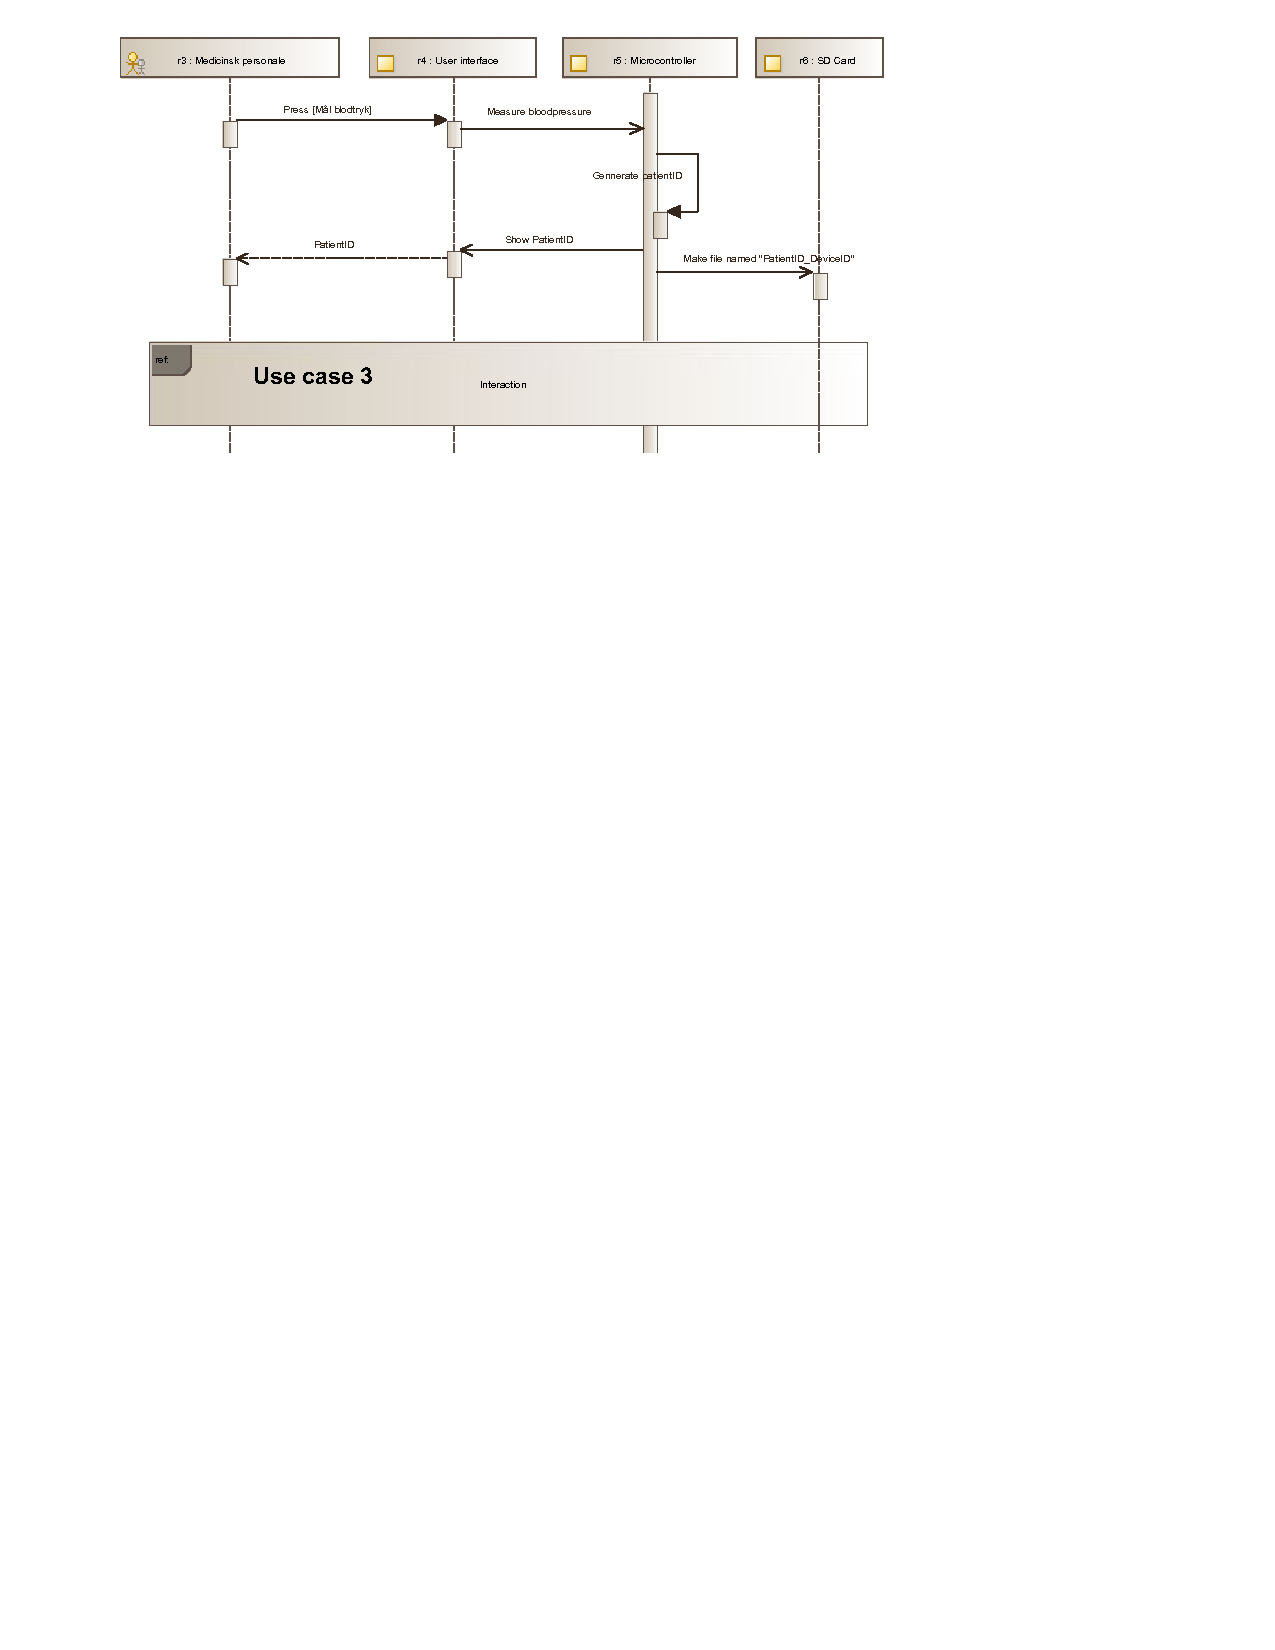
\includegraphics[width=\textwidth]{SystemArkitektur/pdfs/SD_UC2-crop.pdf}
\caption{Sekvens diagram over forløb i use case 2}
\end{figure}
\newpage

\subsection{Mål blodtryk - UC3}
\begin{figure}[H]
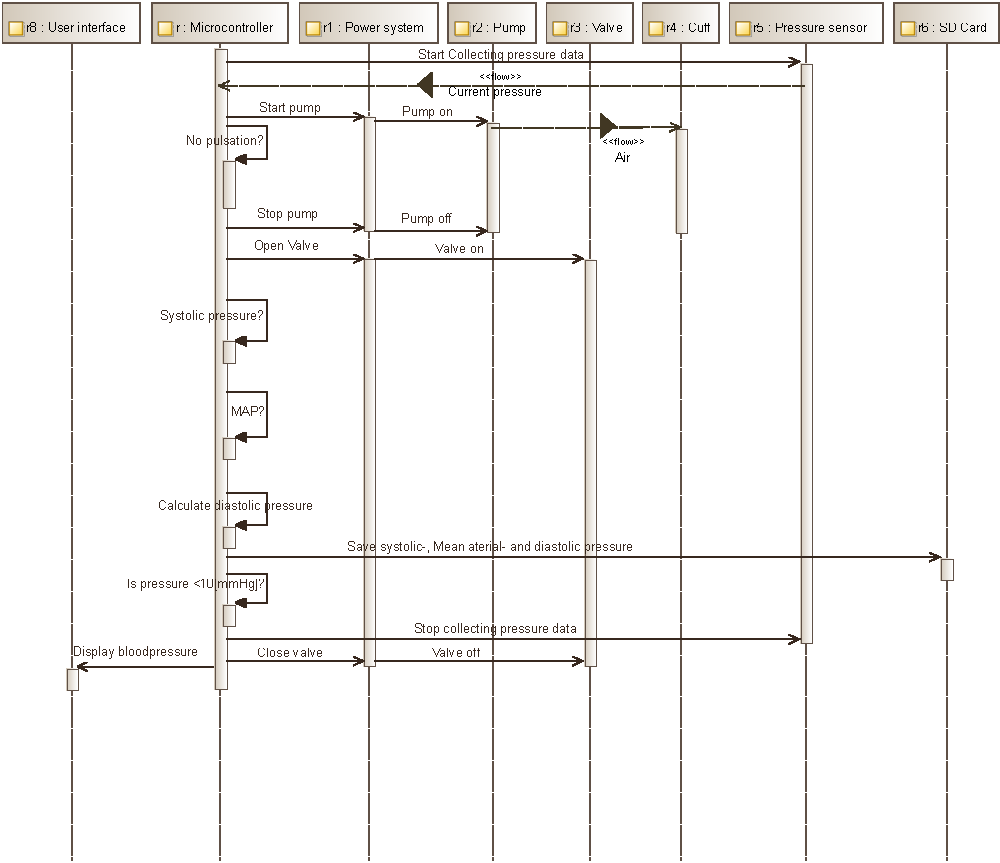
\includegraphics[width=\textwidth]{SystemArkitektur/pdfs/SD_UC3-crop.pdf}
\caption{Sekvens diagram over forløb i use case 3}
\end{figure}
\newpage

\subsection{Overfør data - UC4}
\begin{figure}[H]
\begin{center}
	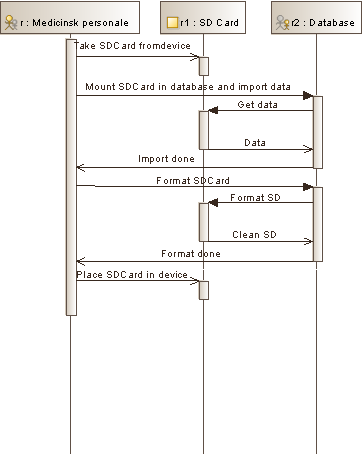
\includegraphics[width=0.60\textwidth]{SystemArkitektur/pdfs/SD_UC4-crop.pdf}
	\caption{Sekvens diagram over forløb i use case 4}
\end{center}
\end{figure}

\newpage

\subsection{Sikkerhedskontrol med pulsoximeter - UC5}
Denne use case og dets sekvens diagram er afgrænses pga. af problematikker med pulsoximetri som sikkerhedskontrol. For mere information se afsnittet omkring projektafgrænsninger i dokumentationsrapporten. 

\subsection{Okklusionstræning - UC6}
\begin{figure}[H]
	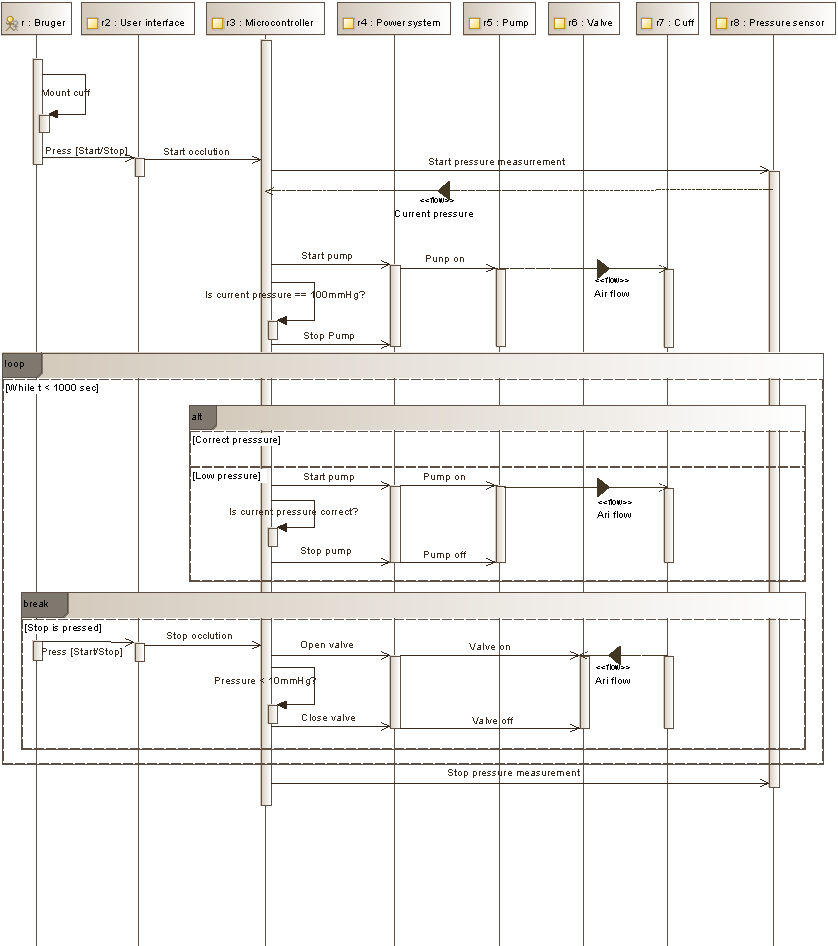
\includegraphics[width=\textwidth]{SystemArkitektur/pdfs/SD_UC6-crop.pdf}
\caption{Sekvens diagram over forløb i use case 6}
\end{figure}
\newpage

\subsection{Afbryd - UC7}
\begin{figure}[H]
	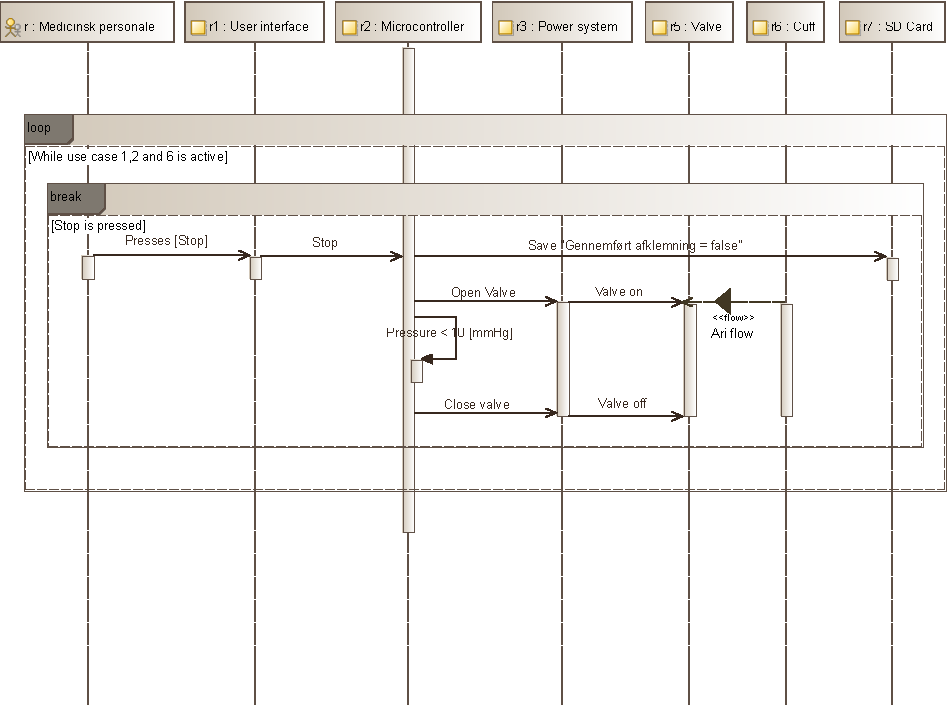
\includegraphics[width=\textwidth]{SystemArkitektur/pdfs/SD_UC7-crop.pdf}
\caption{Sekvens diagram over forløb i use case 7}
\end{figure}
\newpage

\subsection{Setup - UC8}
\begin{figure}[H]
	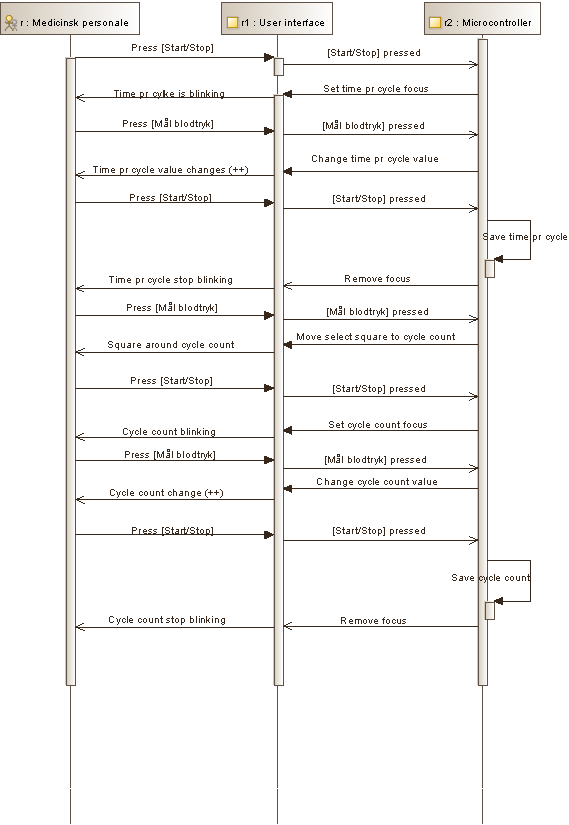
\includegraphics[width=\textwidth]{SystemArkitektur/pdfs/SD_UC8-crop.pdf}
\caption{Sekvens diagram over forløb i use case 8}
\end{figure}
\newpage
